\documentclass{minimal}
\usepackage[a4paper,margin=1cm]{geometry}
\usepackage{tikz}
\usepackage{verbatim}
\begin{document}
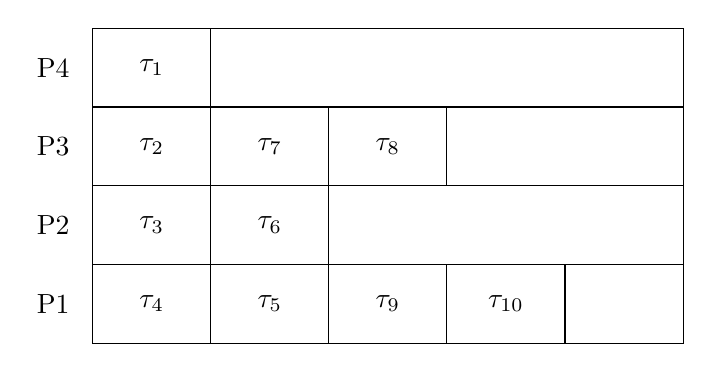
\begin{tikzpicture}
\node at (-0.5,0.5) {P1};
\node at (-0.5,1.5) {P2};
\node at (-0.5,2.5) {P3};
\node at (-0.5,3.5) {P4};
\draw (0,0) rectangle (1.5,1) node[pos=.5] {$\tau_4$};
\draw (0,1) rectangle (1.5,2) node[pos=.5] {$\tau_3$};
\draw (0,2) rectangle (1.5,3) node[pos=.5] {$\tau_2$};
\draw (0,3) rectangle (1.5,4) node[pos=.5] {$\tau_1$};

\draw (1.5,0) rectangle (3,1) node[pos=.5] {$\tau_5$};
\draw (1.5,1) rectangle (3,2) node[pos=.5] {$\tau_6$};
\draw (1.5,2) rectangle (3,3) node[pos=.5] {$\tau_7$};

\draw (3,0) rectangle (4.5,1) node[pos=.5] {$\tau_9$};
\draw (3,2) rectangle (4.5,3) node[pos=.5] {$\tau_8$};

\draw (4.5,0) rectangle (6,1) node[pos=.5] {$\tau_{10}$};
\draw (0,0) rectangle (7.5,4);
\draw (0,0) rectangle (7.5,4);
\draw (0,0) rectangle (7.5,3);
\draw (0,0) rectangle (7.5,2);
\draw (0,0) rectangle (7.5,1);
\end{tikzpicture}
\end{document}